\section{Objetivos}
\begin{itemize}
    \item Estudiar el comportamiento del voltímetro y amperímetro en un circuito genérico para comprender sus funciones y limitaciones.
    \item Medir la corriente y la diferencia de potencial en diferentes tramos de un circuito para analizar la distribución de la tensión y la corriente en configuraciones de resistencias en serie y en paralelo.
    \item Identificar y comprender las características y las diferencias entre las conexiones de resistencias en serie y en paralelo, evaluando cómo estas configuraciones afectan las propiedades eléctricas del sistema.
\end{itemize}

\section{Marco Teórico}
En este laboratorio, se exploran los fundamentos de los circuitos eléctricos a través del estudio de resistencias conectadas en serie y en paralelo. Los conceptos de voltaje (\( V \)), corriente (\( I \)), y resistencia (\( R \)) son centrales en el análisis de circuitos. La ley de Ohm, que establece que \( V = IR \), es fundamental para entender cómo varían el voltaje y la corriente a través de resistencias.

\subsection{Resistencias en Serie}
En una configuración en serie, las resistencias se conectan una tras otra, formando un único camino para el flujo de corriente. La corriente en un circuito serie es la misma a través de cada componente, pero el voltaje total se divide entre las resistencias. La resistencia total, \( R_{total} \), se calcula sumando las resistencias individuales:
\[
R_{total} = R_1 + R_2 + \cdots + R_n
\]
Esta configuración demuestra que el voltaje aplicado en un circuito en serie se distribuye entre las resistencias de acuerdo con sus valores.

\subsection{Resistencias en Paralelo}
En un circuito paralelo, las terminales de todas las resistencias están conectadas a un mismo par de nodos, creando múltiples caminos para la corriente. La diferencia de potencial a través de cada resistencia en paralelo es la misma, y la corriente total del circuito es la suma de las corrientes a través de cada resistencia. La resistencia total en un circuito paralelo se calcula usando la inversa de la suma de las inversas de cada resistencia individual:
\[
\frac{1}{R_{total}} = \frac{1}{R_1} + \frac{1}{R_2} + \cdots + \frac{1}{R_n}
\]
Esta fórmula es crucial para entender cómo la adición de más caminos en un circuito reduce la resistencia total y aumenta la corriente.

Estos principios son esenciales para el diseño y análisis de circuitos eléctricos, permitiendo predecir cómo se comportarán los circuitos bajo diferentes configuraciones y condiciones de carga.


\section{Análisis y discusión: Montaje 1 Resistencias en Serie}

\subsection{Conecte el circuito de la Figura 2}
\textbf{Conecte el circuito de la siguiente figura:}

\begin{figure}[H]
    \centering
    \begin{subfigure}[b]{\textwidth}
        \centering
        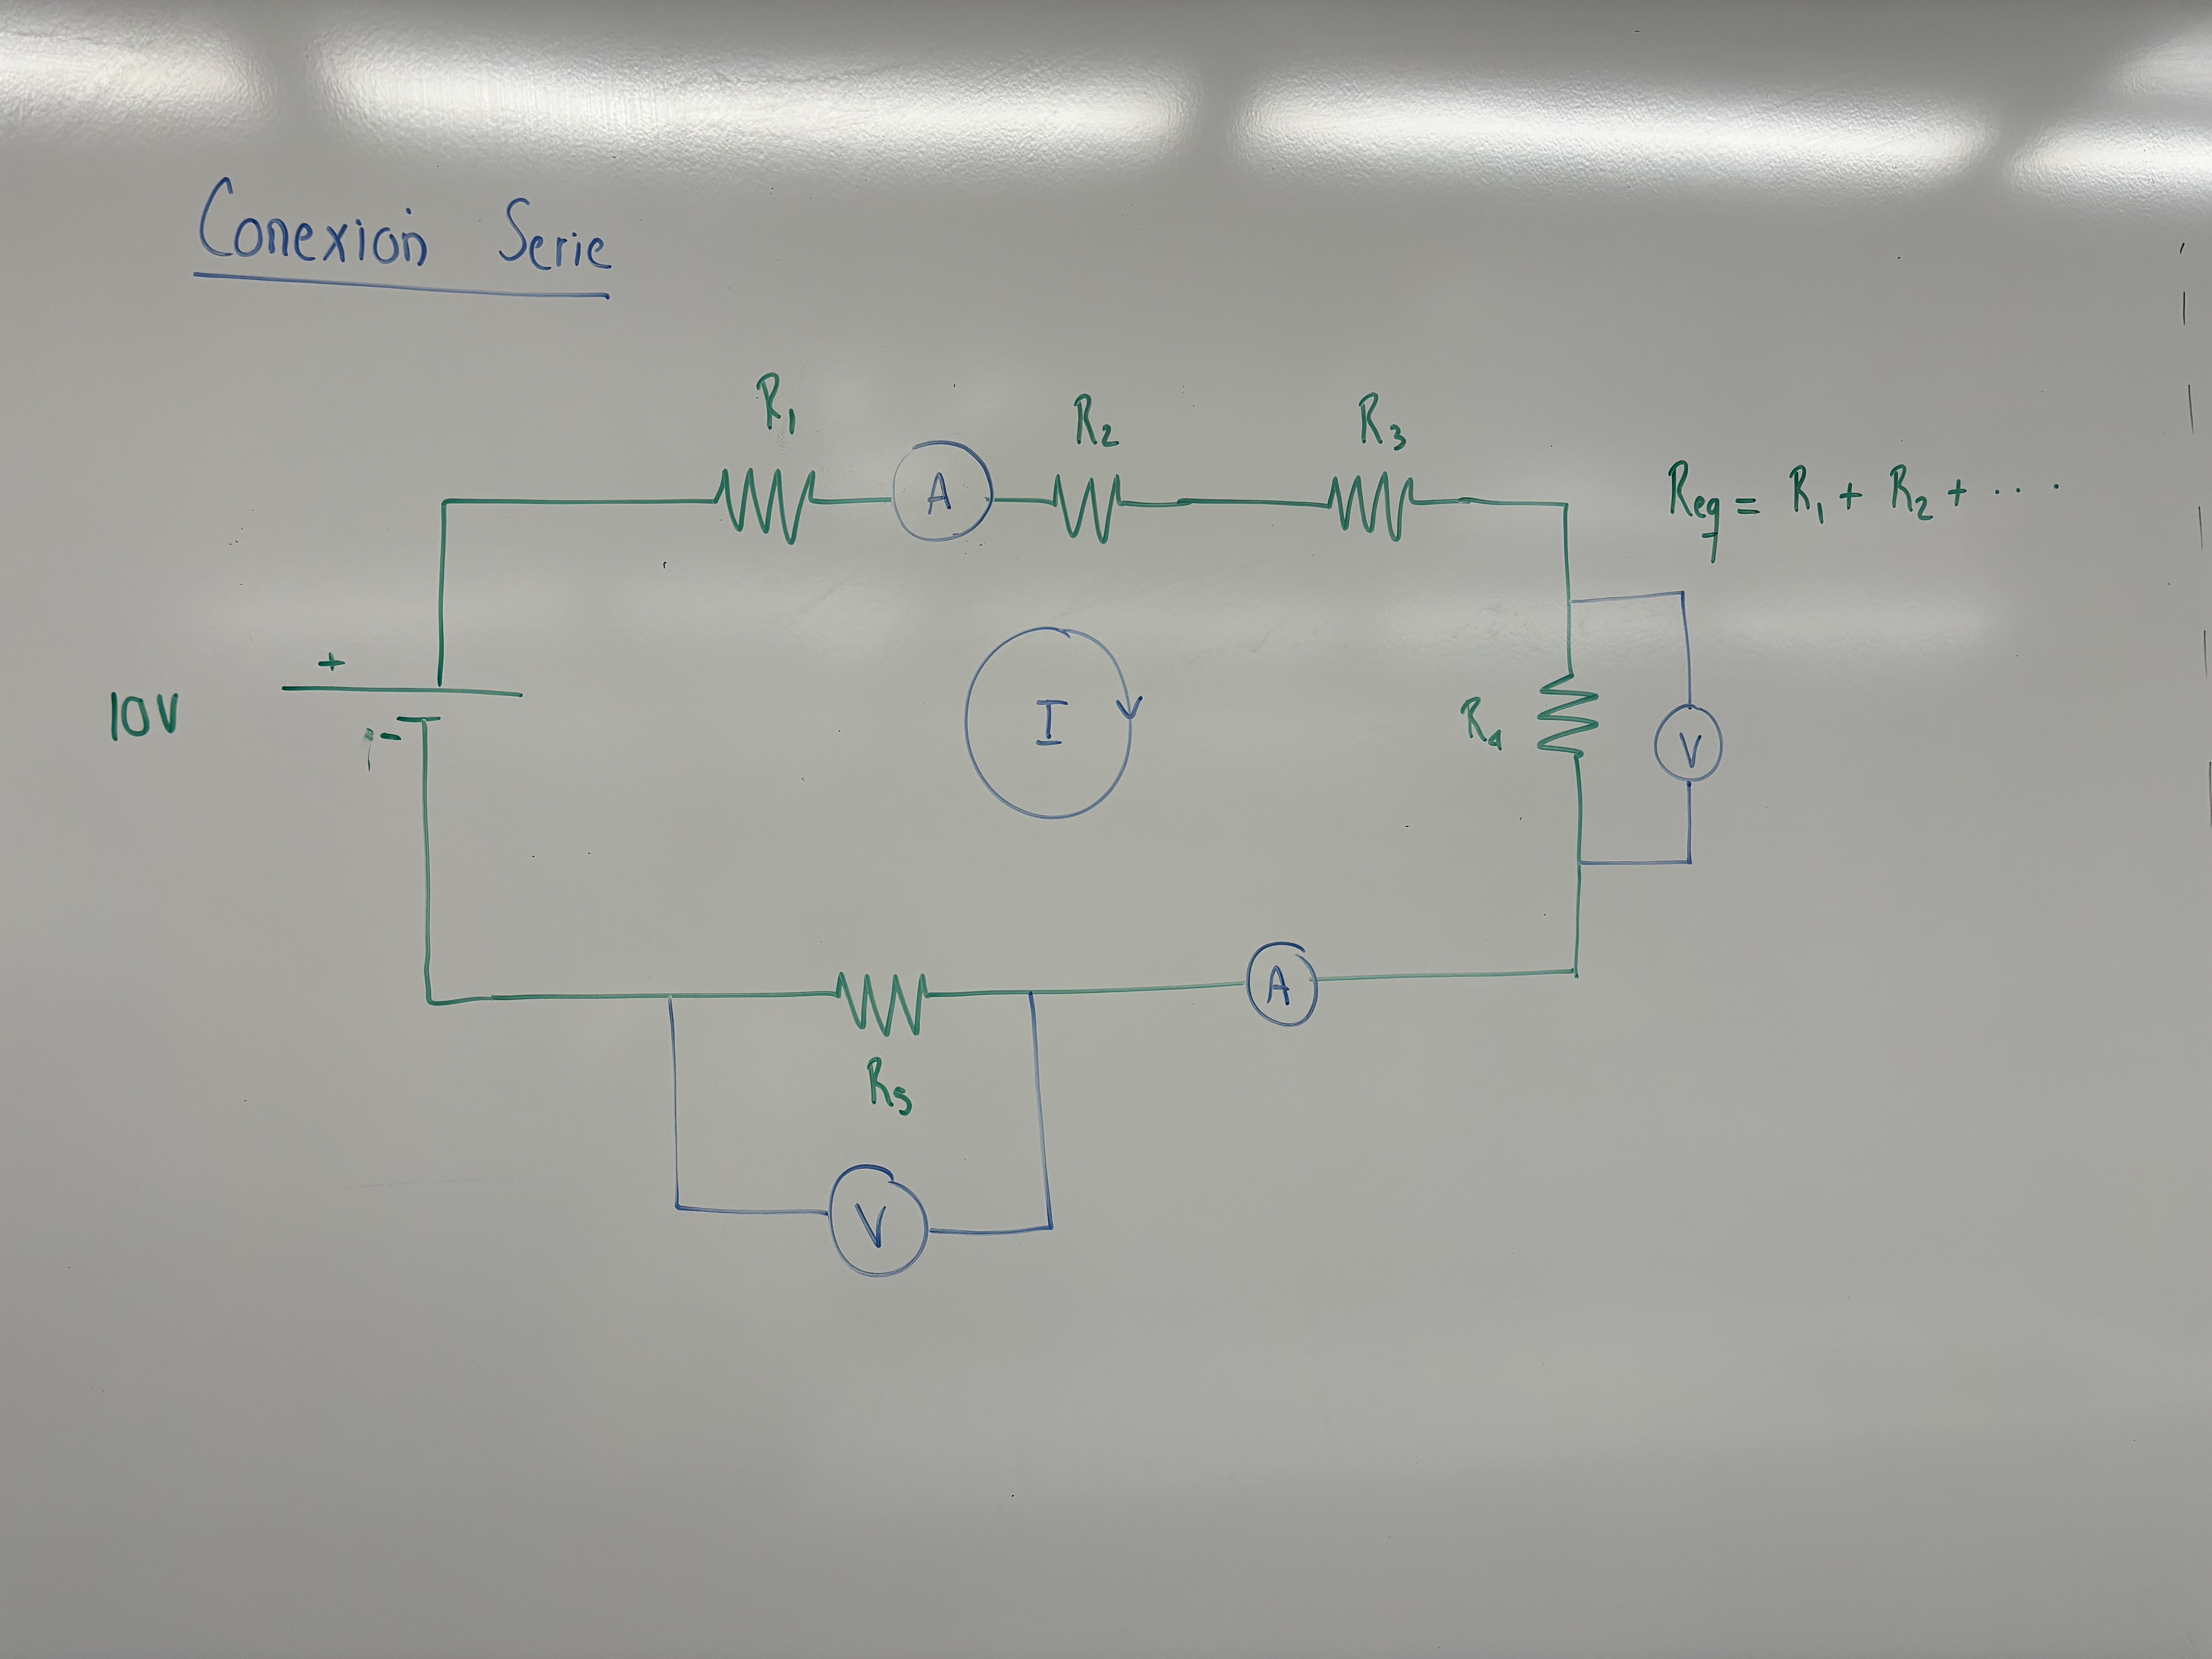
\includegraphics[width=0.8\textwidth]{Figures/1. Content/ConexionSerie.jpg}
        \caption{Conexión en Serie}
        \label{fig: Conexion Serie}
    \end{subfigure}
    \hfill
\end{figure}

Aunque es importante recordar que ambos montajes (Conexión en Serie y Conexión
Paralelo) tienen la siguiente configuración u orden de los resistores
(actualmente estamos usando la configuración para la mesa 3-B):

\begin{figure}[H]
    \centering
    \begin{subfigure}[b]{\textwidth}
        \centering
        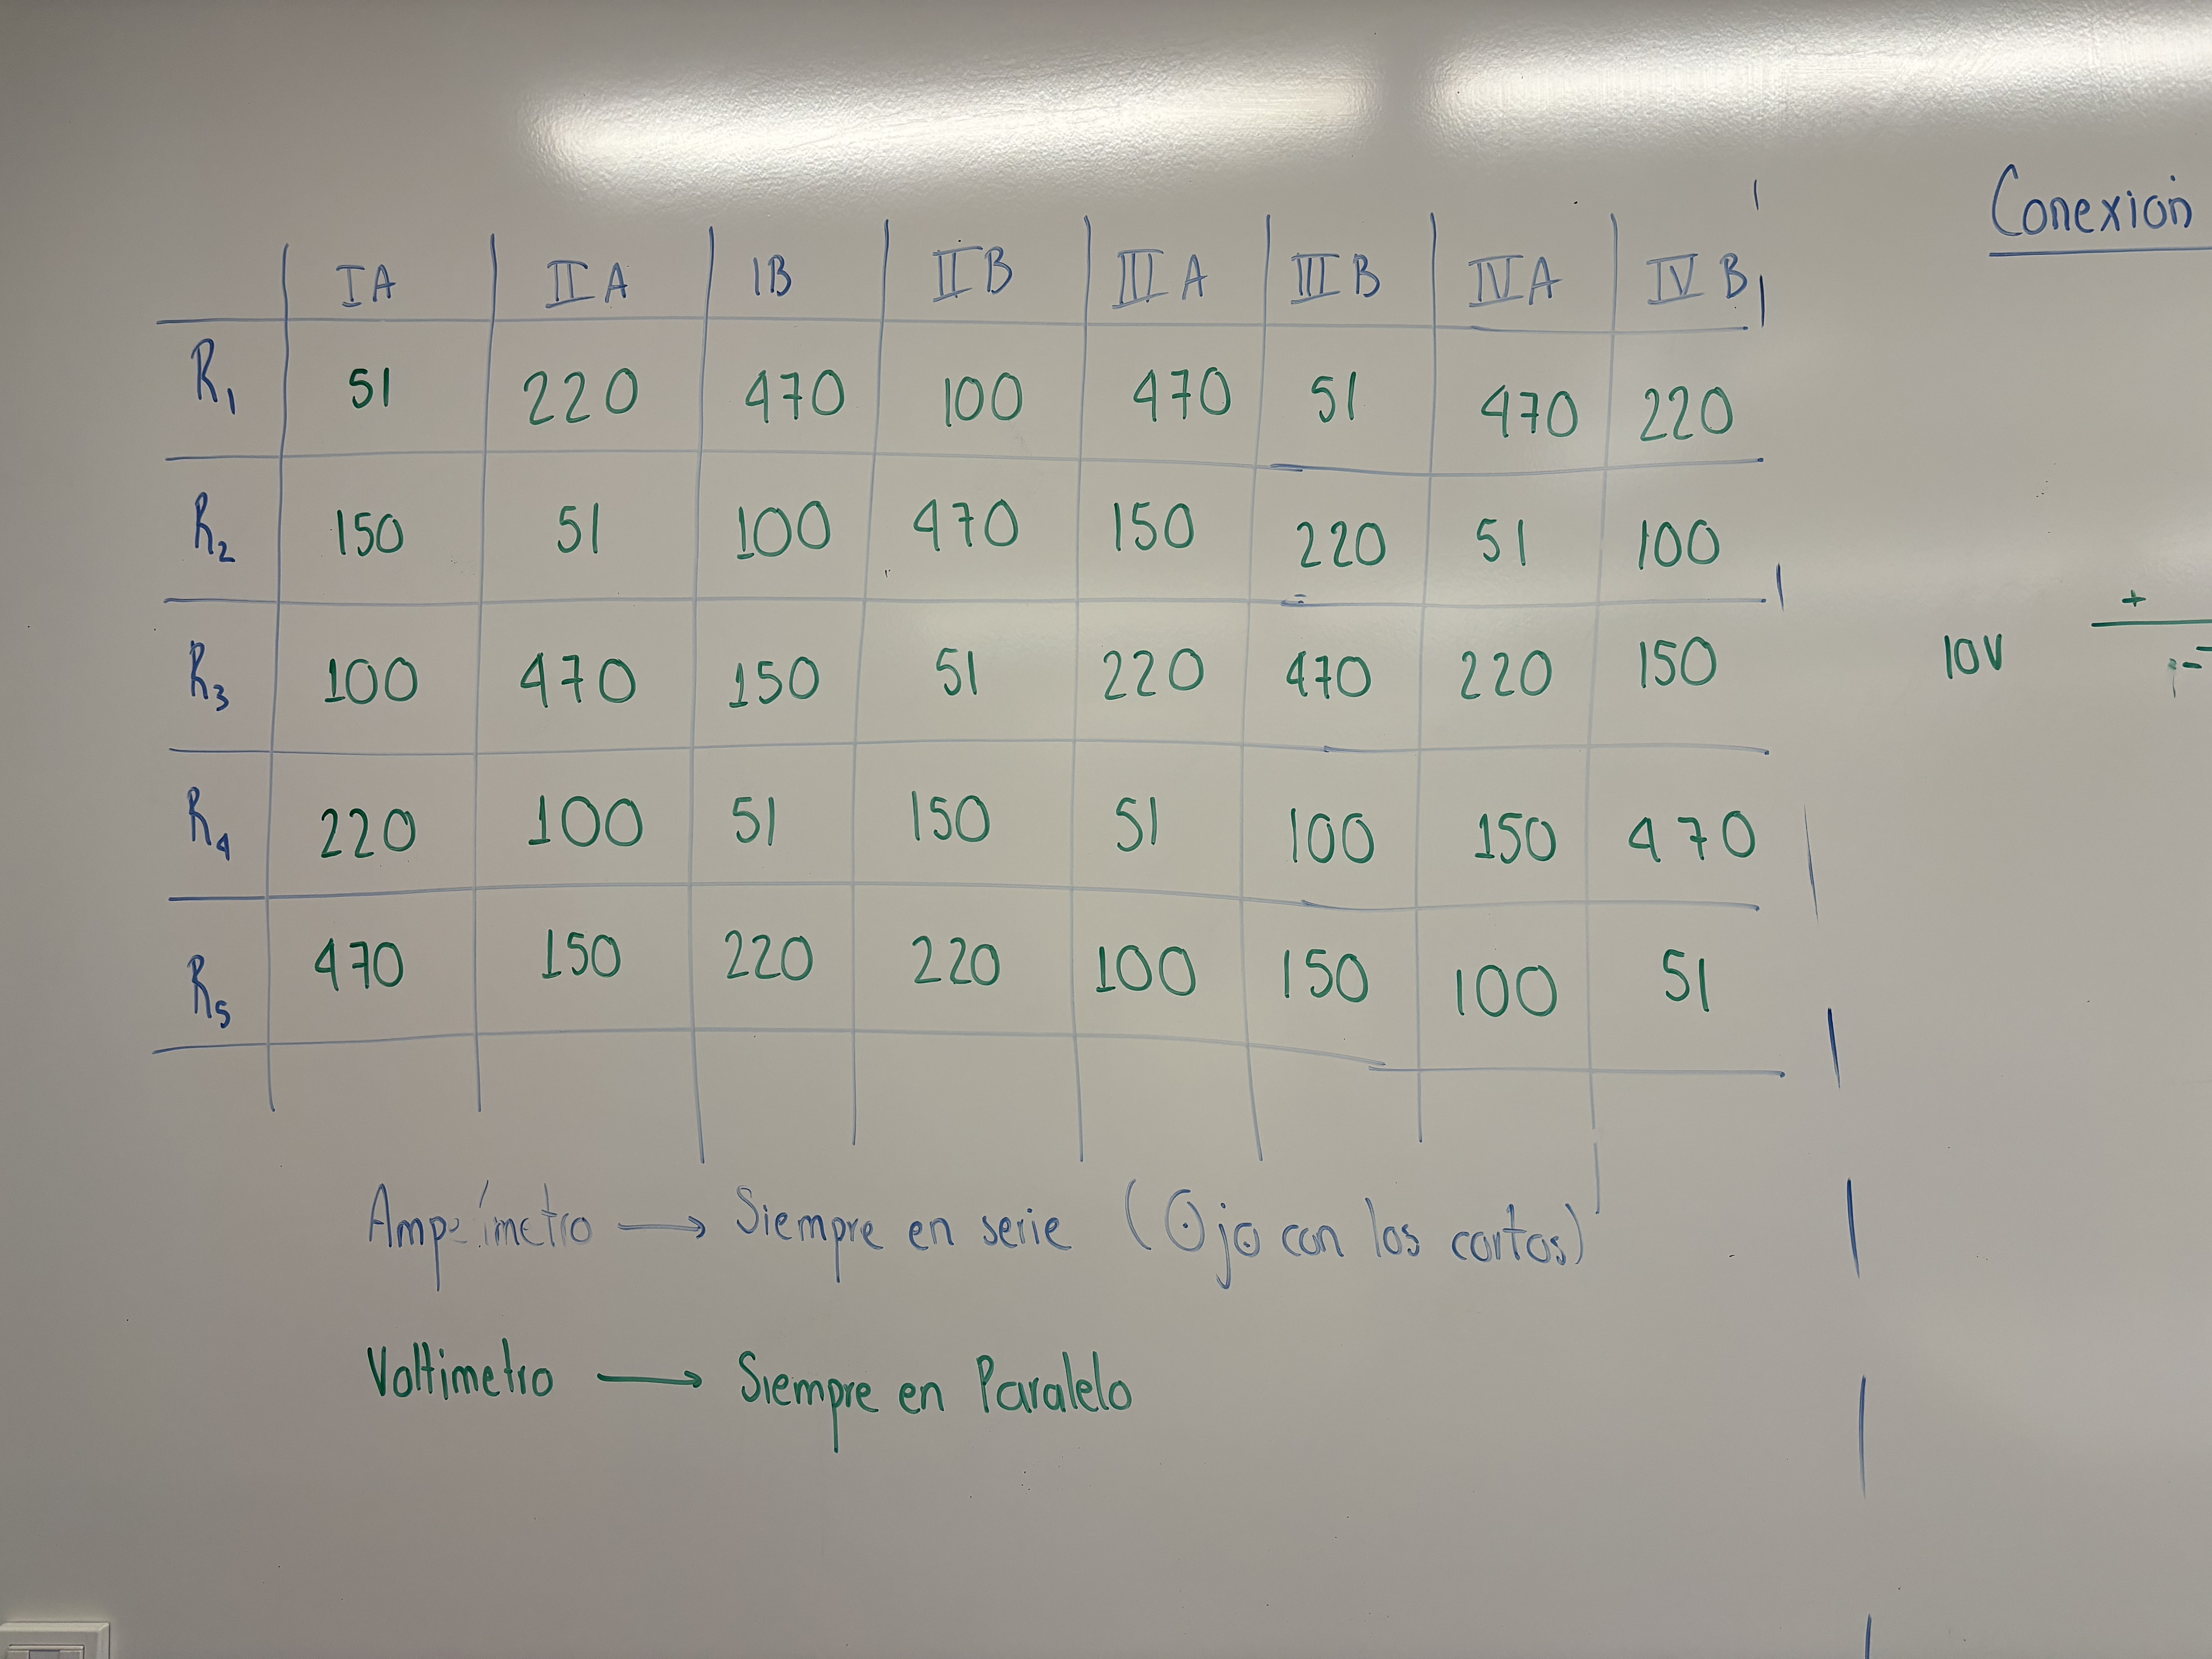
\includegraphics[width=0.8\textwidth]{Figures/1. Content/OrdenResistencias.jpg}
        \caption{Orden de las Resistencias}
        \label{fig: Orden de las Resistencias}
    \end{subfigure}
    \hfill
\end{figure}

\subsection{Significado de tolerancia}
\textbf{¿Qué significado tiene la tolerancia de una resistencia?}
La tolerancia de una resistencia indica el porcentaje máximo por el cual puede variar el valor real de la resistencia respecto a su valor nominal. Es una medida de la precisión con la que la resistencia fue fabricada y es esencial para aplicaciones que requieren precisión en los valores de los componentes.

\subsection{Concordancia de tolerancia}
\textbf{¿Concuerda la tolerancia de cada resistencia dada por el fabricante con las medidas experimentales?}
Para evaluar si las tolerancias concuerdan, comparamos las diferencias porcentuales entre los valores teóricos y experimentales con el porcentaje de tolerancia especificado por el fabricante. Si estas diferencias están dentro de la tolerancia especificada, entonces concuerdan.
Y en este caso las tolerancias concuerdan porque la diferencia entre ellas está dentro de la tolerancia del 5\%.

\subsection{Reportar Corriente}
\textbf{Calcule y reporte la corriente que fluye por este circuito}
Suponiendo que la tensión aplicada al circuito es de 10.3 V, y utilizando la resistencia equivalente experimental de 999.8 \(\Omega\), la corriente que fluye por el circuito se calcula como:
\[
I = \frac{10.3 \, \text{V}}{999.8 \, \Omega} \approx 0.010302 \, \text{A} \, (\text{o} \, 10.302 \, \text{mA})
\]

\subsection{Medición de Corriente en Puntos a y b}
\textbf{Con el amperímetro mida y reporte la corriente en el punto $a$ (Entre R1 y R2) y en el punto $b$ (Entre R4 y R5), ¿qué puede concluir?}

Las mediciones de la corriente en los puntos a y b del circuito en serie dieron como resultado un valor de 0.011 A para ambos puntos. Este resultado es esperado y confirma la propiedad fundamental de los circuitos en serie: la corriente es constante en todos los puntos del circuito. Este valor medido también está en concordancia con el valor calculado teóricamente, que era aproximadamente 0.0103 A, demostrando la uniformidad y la continuidad de la corriente a través de todo el circuito. Esto valida tanto la precisión de las mediciones experimentales como la integridad del circuito bajo prueba.

\section{Procedimiento Experimental y Resultados: Montaje 2 Resistencias en Paralelo}

\subsection{Conecte el circuito de la Figura 3}
\textbf{Conecte el circuito de la siguiente figura:}
\begin{figure}[H]
    \centering
    \begin{subfigure}[b]{\textwidth}
        \centering
        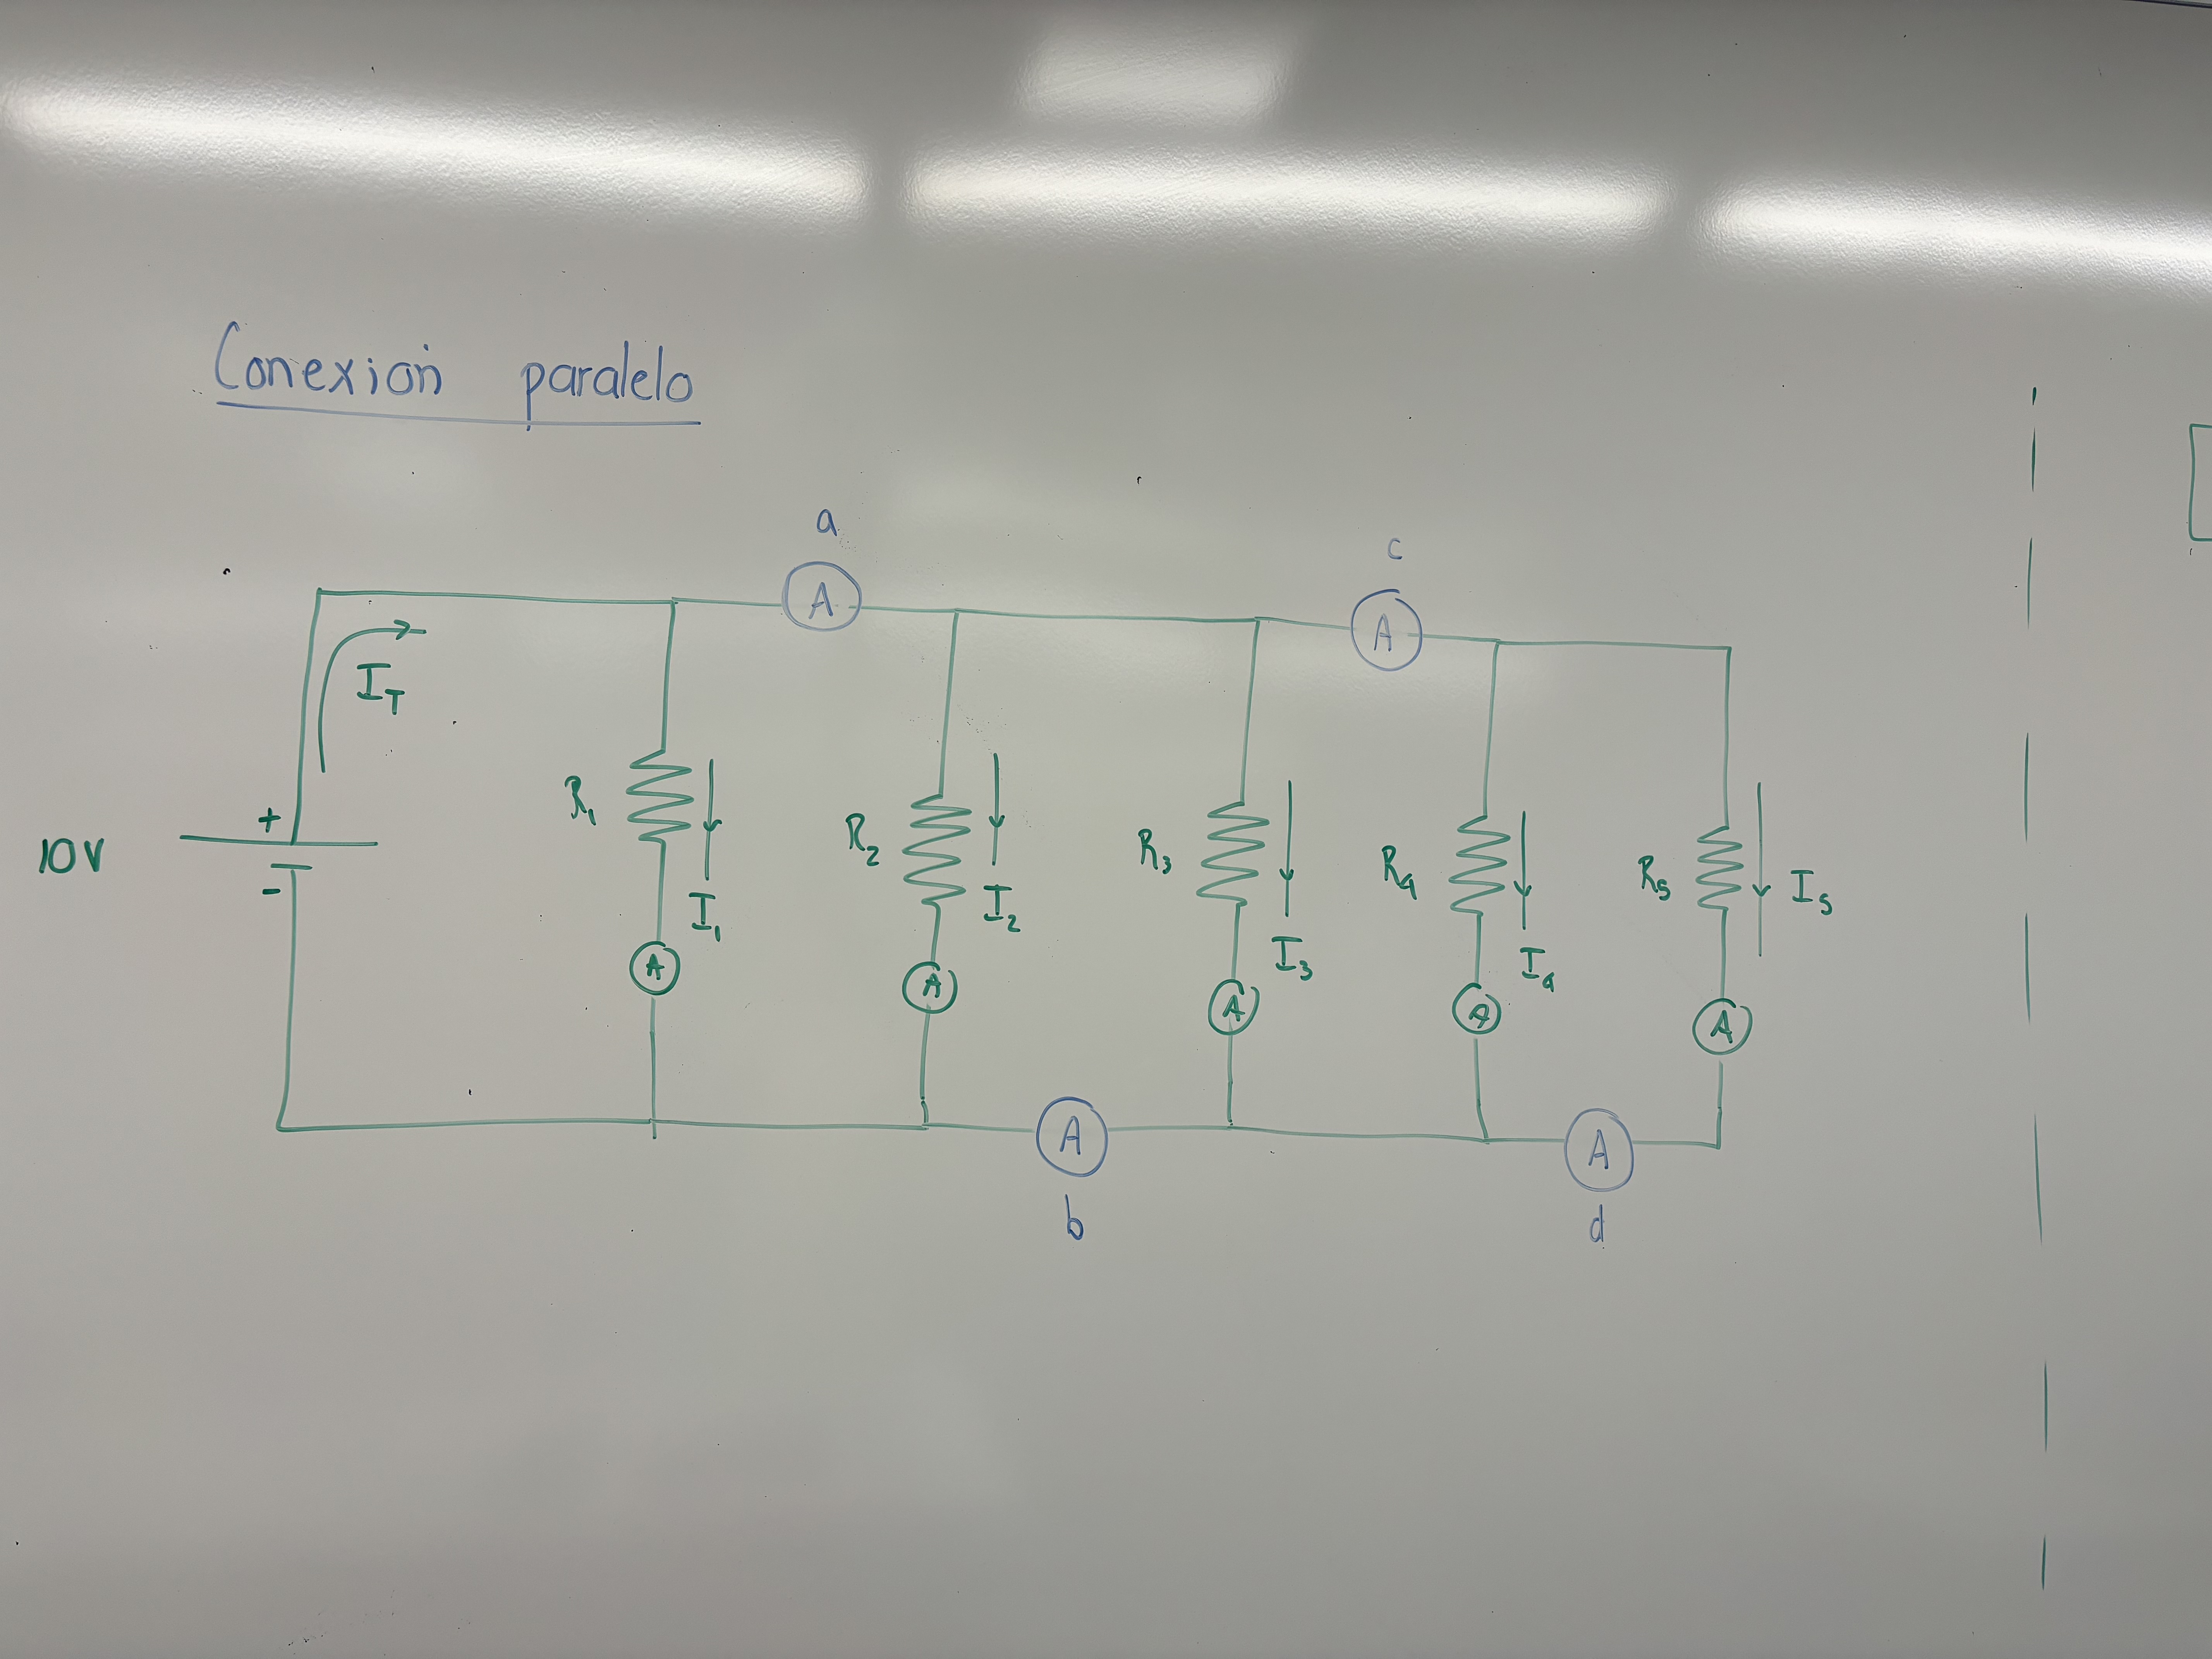
\includegraphics[width=0.8\textwidth]{Figures/1. Content/ConexionParalelo.jpg}
        \caption{Conexión en Paralelo}
        \label{fig: Conexion Paralelo}
    \end{subfigure}
    \hfill
\end{figure}

\subsection{Corriente en cada resistor}
\textbf{Con el amperímetro mida y reporte la corriente entregada por la fuente y a través de cada resistor:}

La corriente medida a través de cada resistor se presenta en la siguiente tabla:

\begin{table}[h]
\centering
\begin{tabular}{|c|c|c|c|c|c|}
\hline
\(I (A)\) & \(I_1 (A)\) & \(I_2 (A)\) & \(I_3 (A)\) & \(I_4 (A)\) & \(I_5 (A)\) \\ \hline
$0.471$     & $0.205$       & $0.052$       & $0.025$       & $0.116$       & $0.076$       \\ \hline
\end{tabular}
\caption{Corrientes medidas en cada punto del circuito.}
\label{tab:current_measurements}
\end{table}

Esta tabla muestra de manera organizada la distribución de la corriente a través de cada resistor, además de la corriente total medida directamente de la fuente.

\subsection{Cálculo de la Suma de Corrientes}
\textbf{Calcule \(I_1 + I_2 + I_3 + I_4 + I_5 = \_\_\_\_\_ \)}
La suma de las corrientes a través de cada resistor se calculó como:
\[
I_1 + I_2 + I_3 + I_4 + I_5 = 0.205 + 0.052 + 0.025 + 0.116 + 0.076 = 0.474 \, \text{A}
\]
Esta suma es muy cercana al valor de corriente total medido, \(0.471 \, \text{A}\), y está dentro de lo esperado considerando posibles errores de medición.

\subsection{Comparación de la Corriente Total}
\textbf{¿Cómo es la corriente entregada por la fuente comparada con el resultado de 2.2? Explique.}
La corriente total entregada por la fuente, \(0.471 \, \text{A}\), es casi idéntica a la suma de las corrientes a través de cada componente del circuito, \(0.474 \, \text{A}\). Esta pequeña discrepancia entre los valores puede atribuirse a errores menores en la medición y la precisión del amperímetro. Este resultado confirma la ley de conservación de la carga, que postula que la corriente total en un circuito cerrado debe ser constante y equivalente a la suma de las corrientes que fluyen a través de cada componente del circuito.

\subsection{Corriente nodo $a$}
\textbf{¿Qué valor tiene la corriente que sale del nodo $a$?} \underline{$0.219$}


\subsection{Corriente nodo $b$}
\textbf{¿Qué valor tiene la corriente que sale del nodo $a$?} \underline{$0.218$}


\subsection{Corriente nodo $c$}
\textbf{¿Qué valor tiene la corriente que sale del nodo $a$?} \underline{$0.193$}


\subsection{Corriente nodo $d$}
\textbf{¿Qué valor tiene la corriente que sale del nodo $a$?} \underline{$0.115$}

\subsection{Voltaje en cada resistor}
\textbf{Mida y reporte el voltaje en cada resistor:}

El voltaje medido a través de cada resistor se presenta en la siguiente tabla:

\begin{table}[h]
\centering
\begin{tabular}{|c|c|c|c|c|c|}
\hline
\(V_{Fuente} (V)\) & \(V_1 (V)\) & \(V_2 (V)\) & \(V_3 (V)\) & \(V_4 (V)\) & \(V_5 (V)\) \\ \hline
$10.3$     & $10.42$       & $10.39$       & $10.48$       & $10.46$       & $10.45$       \\ \hline
\end{tabular}
\caption{Voltajes medidas en cada punto del circuito.}
\label{tab:volt_measurements}
\end{table}

\subsection{Voltaje en Cada Resistor Comparado con la Fuente}
\textbf{¿Cómo es el voltaje en cada resistor comparado con el voltaje entregado por la fuente? Explique.}
Los voltajes medidos en cada resistor (aproximadamente 10.4 V para cada uno) son sorprendentemente similares y ligeramente superiores al voltaje teórico de la fuente (10 V) y al experimental medido directamente (10.3 V). Esto puede atribuirse a pequeños errores de medición o variaciones en la carga real en el momento de las mediciones. El hecho de que todos los resistores muestren voltajes similares también indica que la caída de tensión a lo largo del circuito es uniforme, lo que es típico en circuitos en serie donde la misma corriente fluye a través de cada componente.

\section{Interacción de las Resistencias Internas de los Equipos de Medida}
\textbf{Sabiendo que tanto el voltímetro como el amperímetro son equipos que poseen resistencias internas, ¿cuál es la razón para que estas no interactúen con la medida?}
Los amperímetros están diseñados para tener una resistencia interna muy baja para minimizar su impacto en el circuito cuando se conectan en serie, lo cual podría alterar la corriente que se está midiendo. Los voltímetros, por otro lado, tienen una resistencia interna muy alta para evitar la extracción de corriente significativa del punto de medición, lo que podría afectar la tensión que se está midiendo.

\section{Importancia de Resistencias y Condensadores Equivalentes}
\textbf{¿Qué importancia tiene poder tener resistencias o condensadores equivalentes en un circuito?}
Las resistencias y condensadores equivalentes permiten simplificar el análisis y diseño de circuitos complejos. Al reemplazar un grupo de componentes en serie o paralelo por un único componente equivalente, se puede calcular más fácilmente el comportamiento general del circuito, especialmente en los casos de análisis de respuesta en frecuencia y carga dinámica.

\section{Conexión de Amperímetros en Serie}
\textbf{¿Por qué los amperímetros deben conectarse en serie en el circuito?}
Los amperímetros deben conectarse en serie para poder medir la totalidad de la corriente que fluye a través del circuito. Si se conectaran de otra manera, como en paralelo, podrían cortocircuitar el circuito en el punto de medición o no medir correctamente la corriente que pasa por otros componentes del circuito.

\section{Procedimiento Experimental y Resultados: Montaje 3 Simulaciones en TinkerCad}

\subsection{Conexiones en Serie}
\begin{figure}[H]
    \centering
    \begin{minipage}{0.45\textwidth}
      \centering
      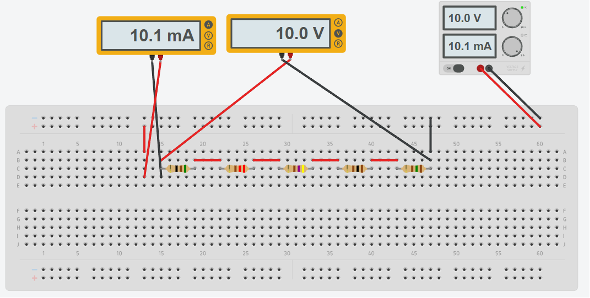
\includegraphics[width=\textwidth]{Figures/1. Content/simulation/serie.png}
      \captionof{figure}{Simulación Conexión en Serie}
      \label{fig: Simulacion Conexion Serie}
    \end{minipage}
    \hfill
    \begin{minipage}{0.45\textwidth}
      \centering
      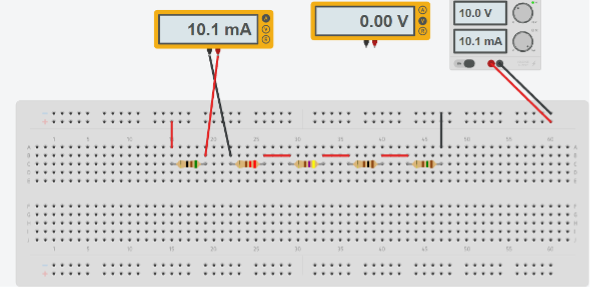
\includegraphics[width=\textwidth]{Figures/1. Content/simulation/serieA1.png}
      \captionof{figure}{Simulación Conexión en Serie $I_{R_1-R_2}$}
      \label{fig: Simulacion Conexion Serie A1}
    \end{minipage}
    \hfill
    \begin{minipage}{0.45\textwidth}
      \centering
      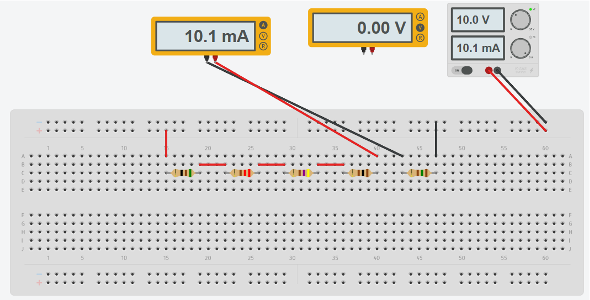
\includegraphics[width=\textwidth]{Figures/1. Content/simulation/serieA2.png}
      \captionof{figure}{Simulación Conexión en Serie $I_{R_4-R_5}$}
      \label{fig: Simulacion Conexion Serie A2}
    \end{minipage}
    \hfill
    \begin{minipage}{0.45\textwidth}
      \centering
      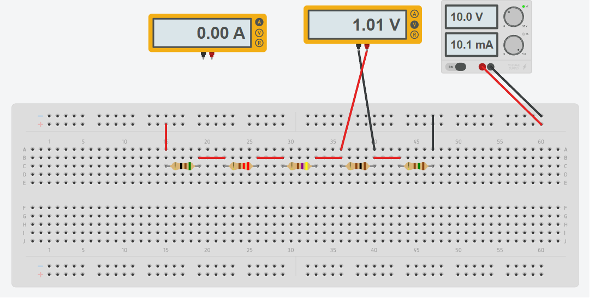
\includegraphics[width=\textwidth]{Figures/1. Content/simulation/serieV1.png}
      \captionof{figure}{Simulación Conexión en Serie $V_{R_4}$}
      \label{fig: Simulacion Conexion Serie V1}
    \end{minipage}
    \hfill
    \begin{minipage}{0.45\textwidth}
      \centering
      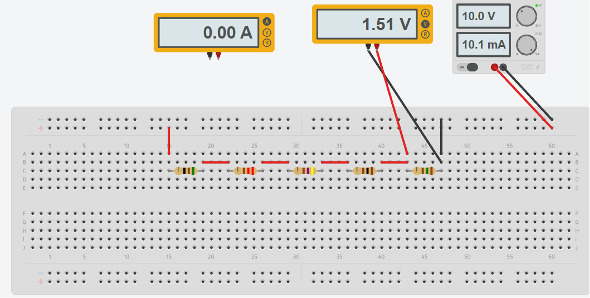
\includegraphics[width=\textwidth]{Figures/1. Content/simulation/serieV2.png}
      \captionof{figure}{Simulación Conexión en Serie $V_{R_5}$}
      \label{fig: Simulacion Conexion Serie V2}
    \end{minipage}
\end{figure}

\subsection{Conexiones en Paralelo}
\begin{figure}[H]
    \centering
    \begin{minipage}{0.45\textwidth}
      \centering
      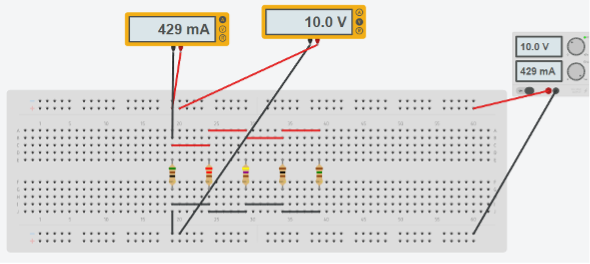
\includegraphics[width=\textwidth]{Figures/1. Content/simulation/paralelo.png}
      \captionof{figure}{Simulación Conexión en Paralelo}
      \label{fig: Simulacion Conexion Paralelo}
    \end{minipage}
    \hfill
    \begin{minipage}{0.45\textwidth}
      \centering
      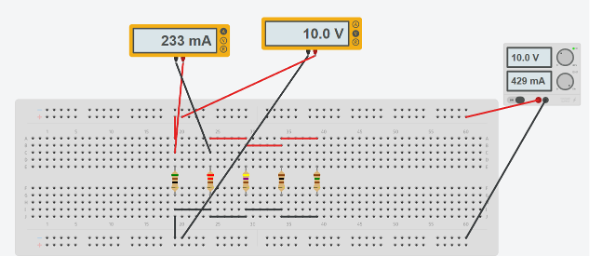
\includegraphics[width=\textwidth]{Figures/1. Content/simulation/paraleloA.png}
      \captionof{figure}{Simulación Conexión en Paralelo en nodo $a$}
      \label{fig: Simulacion Conexion Paralelo A}
    \end{minipage}
    \hfill
    \begin{minipage}{0.45\textwidth}
      \centering
      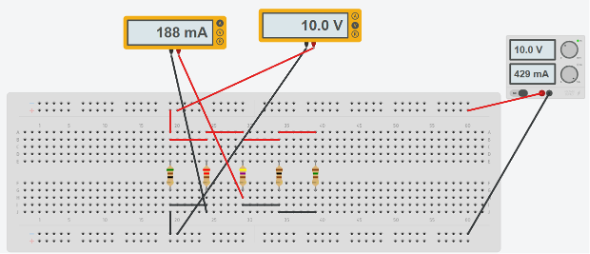
\includegraphics[width=\textwidth]{Figures/1. Content/simulation/paraleloB.png}
      \captionof{figure}{Simulación Conexión en Paralelo en nodo $b$}
      \label{fig: Simulacion Conexion Paralelo B}
    \end{minipage}
    \hfill
    \begin{minipage}{0.45\textwidth}
      \centering
      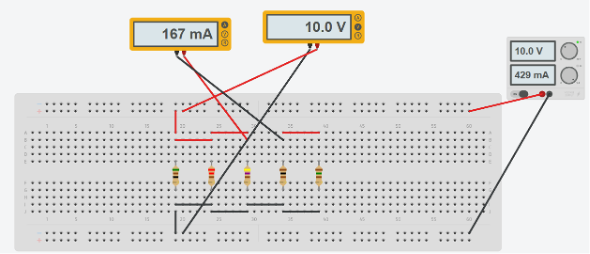
\includegraphics[width=\textwidth]{Figures/1. Content/simulation/paraleloC.png}
      \captionof{figure}{Simulación Conexión en Paralelo en nodo $c$}
      \label{fig: Simulacion Conexion Paralelo C}
    \end{minipage}
    \hfill
    \begin{minipage}{0.45\textwidth}
      \centering
      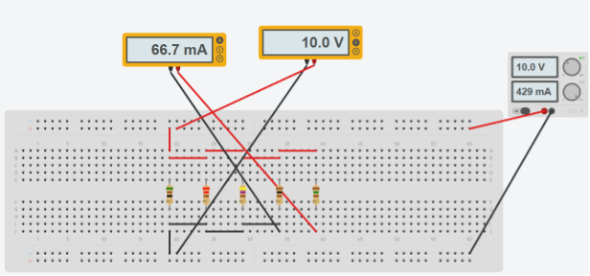
\includegraphics[width=\textwidth]{Figures/1. Content/simulation/paraleloD.png}
      \captionof{figure}{Simulación Conexión en Paralelo en nodo $d$}
      \label{fig: Simulacion Conexion Paralelo D}
    \end{minipage}
    \hfill
    \begin{minipage}{0.45\textwidth}
      \centering
      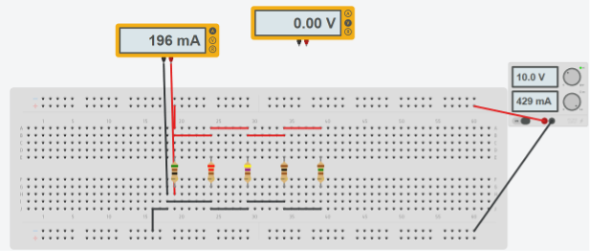
\includegraphics[width=\textwidth]{Figures/1. Content/simulation/paraleloAR1.png}
      \captionof{figure}{Simulación Conexión en Paralelo $I_{R_1}$}
      \label{fig: Simulacion Conexion Paralelo IR1}
    \end{minipage}
    \hfill
    \begin{minipage}{0.45\textwidth}
      \centering
      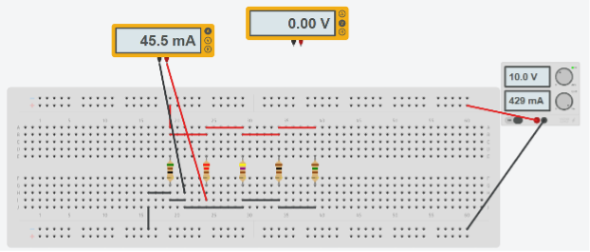
\includegraphics[width=\textwidth]{Figures/1. Content/simulation/paraleloAR2.png}
      \captionof{figure}{Simulación Conexión en Paralelo $I_{R_2}$}
      \label{fig: Simulacion Conexion Paralelo IR2}
    \end{minipage}
    \hfill
    \begin{minipage}{0.45\textwidth}
      \centering
      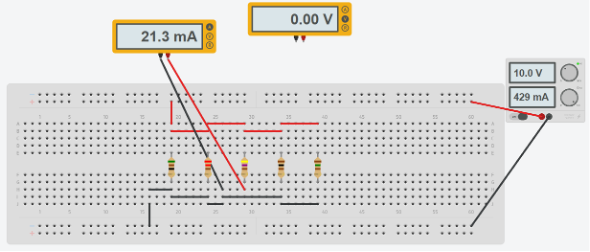
\includegraphics[width=\textwidth]{Figures/1. Content/simulation/paraleloAR3.png}
      \captionof{figure}{Simulación Conexión en Paralelo $I_{R_3}$}
      \label{fig: Simulacion Conexion Paralelo IR3}
    \end{minipage}
    \hfill
    \begin{minipage}{0.45\textwidth}
      \centering
      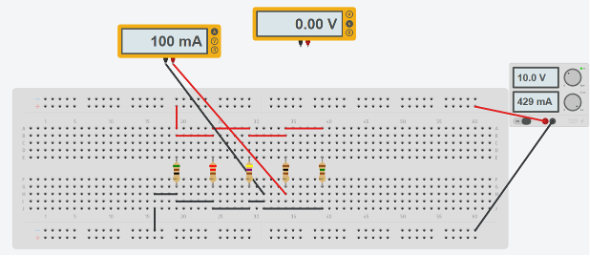
\includegraphics[width=\textwidth]{Figures/1. Content/simulation/paraleloAR4.png}
      \captionof{figure}{Simulación Conexión en Paralelo $I_{R_4}$}
      \label{fig: Simulacion Conexion Paralelo IR4}
    \end{minipage}
    \hfill
    \begin{minipage}{0.45\textwidth}
      \centering
      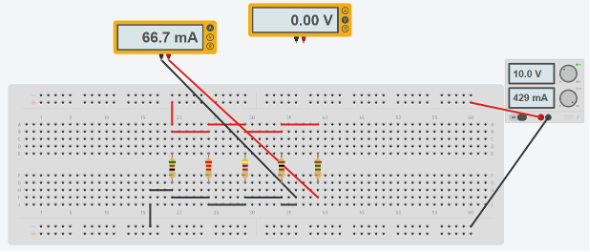
\includegraphics[width=\textwidth]{Figures/1. Content/simulation/paraleloAR5.png}
      \captionof{figure}{Simulación Conexión en Paralelo $I_{R_5}$}
      \label{fig: Simulacion Conexion Paralelo IR5}
    \end{minipage}
\end{figure}


\section{Causas de Error}
Las principales causas de error en este experimento podrían incluir:
\begin{itemize}
    \item Errores de calibración en los instrumentos de medición como amperímetros y voltímetros que podrían haber afectado las mediciones de corriente y voltaje respectivamente.
    \item Resistencias internas de los instrumentos de medición que, aunque diseñadas para minimizar su impacto, pueden introducir pequeñas variaciones en las mediciones.
    \item Variaciones en las resistencias reales respecto a sus valores nominales, lo que podría afectar la distribución de la corriente y el voltaje en el circuito.
    \item Errores en la conexión de los componentes del circuito que podrían haber creado caminos de corriente adicionales o contactos imperfectos.
    \item Influencias ambientales como la temperatura, que puede cambiar las propiedades de los materiales de los componentes, especialmente las resistencias.
\end{itemize}

\section{Conclusiones}
A partir del experimento realizado, se pueden extraer las siguientes conclusiones:
\begin{itemize}
    \item Se confirmó que en un circuito en serie, la corriente es constante a través de cada componente, mientras que la tensión se distribuye entre los componentes en función de su resistencia.
    \item En los circuitos en paralelo, se verificó que la tensión en cada rama es igual a la tensión de la fuente, mientras que la corriente se divide entre las ramas en función de la resistencia de cada una.
    \item Las mediciones experimentales mostraron una buena concordancia con los valores teóricos esperados, aunque con ligeras desviaciones que pueden atribuirse a las causas de error identificadas.
    \item El experimento destacó la importancia de la precisión en la fabricación de los componentes del circuito y la precisión en las técnicas de medición para asegurar la confiabilidad de los resultados experimentales.
    \item Estos resultados refuerzan la comprensión de las leyes fundamentales de los circuitos eléctricos y la importancia de la configuración correcta y el uso adecuado de los instrumentos de medición en prácticas de laboratorio.
\end{itemize}